%-*- coding: UTF-8 -*-
% 勾股定理
% 指定文档类,因为是中文,所以使用ctexart并且用UTF8制定编码
\documentclass[UTF8]{ctexart}
\usepackage{graphicx}
\usepackage{amsmath}
\usepackage{float}
\usepackage{geometry}
% 使用悬挂对齐方方式,整体使用小字号,标题文本使用斜体,对汉字来说,是楷书。
\usepackage[format=hang, font=small, textfont=it]{caption}
% 设定页面使用A6纸大小,版心居中,长宽占页面的0.8倍
\geometry{a6paper, centering, scale=0.8}
% 定理环境是一类环境,需要在导言区做定义
\newtheorem{thm}{定理}
% 以下三页的信息,并不会马上出现在编译结果中,他们要通过使用maketitle才会进行排版
\title{\heiti 杂谈勾股定理}
\author{\kaishu 张三}
\date{\today}
\bibliographystyle{plain}



% 在此行之前的部分称为导言区,导演去通常是用来对文档的性质做一些设置,或者自定义一些命令
% begin和enddocument之间声明了一个documents环境,也就是直接输出的部分。

\begin{document}
% 声明参考文献的格式

% 实际输出论文标题
\maketitle
% 实际输出目录
\tableofcontents
% section表示开始新的一节
\section{勾股定理在现代}\label{sec:first}
 	% 中文中的换行和空格都没有意义,ctex都会为他们自动排版,但是英语不会忽略空格
	西方称勾股定理为毕达哥拉斯定理,将勾股定理的发现归功于公元前 6 世纪的毕达哥拉斯学派\cite{Kline}。该学派得到了一个法则,
	% 使用footnote来获取脚注,大括号内的为传给footnote的参数。
	可以排出可排成直角 三角形三边的三元数组。毕达哥拉斯学派没有书面著作,该定理的严格表述和证明则见于欧几里德\footnote{欧几里德,约公元前 330--275年}
	《几何原本》的命题 47:“直角三角形斜边上的正方 形等于两直角边上的两个正方形之和。”证明是用面积做的。我国《周髀算经》载商高(约公元前 12 世纪) 答周公问:
	% quote环境讲其中的内容单独分行,增加锁进和上下间距排版,以突出有用的部分。
	\begin{quote}
		% 利用zihao来确定字号,kaishu确定字体为楷书。
		\zihao{-5}\kaishu 勾广三,股修四,径隅五。
	\end{quote}
	又载陈子(约公元前 7–6 世纪)答荣方问:
	\begin{quote}
		\zihao{-5}\kaishu 若求邪至日者,以日下为勾,日高为股,勾股各自乘,并而开方除之,得邪至日。
	\end{quote}
	% 引用图1
	都较古希腊更早。后者已经明确道出勾股定理的一 般形式。图\ref{fig:xiantu}是我国古代对勾股定理的一种证明\cite{quanjing}
	
	% figure是插图可以使用的浮动体环境,ht参数表示浮动题可以出现在环境周围的浮动体环境和一页的顶部。
	% 绝大部分情况下,文章中的插图都是用的与这里几乎完全相同的代码插入。
	\begin{figure}[ht]
		\centering
		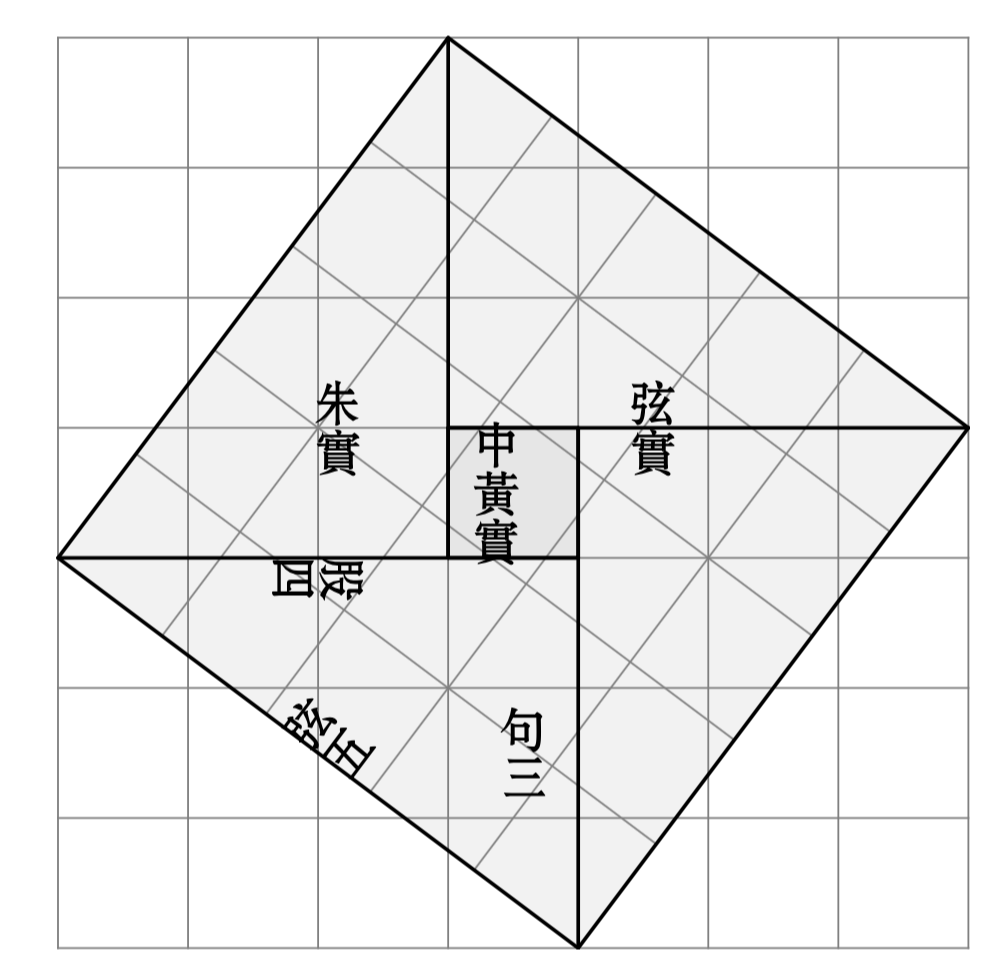
\includegraphics[width=3cm]{goutu.png}
		\caption{宋赵爽在《周髀算经》注中做的弦图(仿制),该图给出了勾股定理一个极具对称美感的证明。}
		% label产生一个标签,使用这个标签可以在文章的其他地方引用\caption产生的编号
		\label{fig:xiantu}
	\end{figure}
\section{勾股定理的近代形式}
	\begin{thm}[勾股定理]
		直角三角形斜边的平方等于两腰的平方和。
		% 使用空行分段,单个换行不会使他分段。
		可以用符号语言表示为:$\angle C = 90^\circ$,则有
		% 由于单独划出来一个公式区域,所以不用空行分段。	
		\begin{equation}\label{eq:gougu}
			AB^2 = BC^2 + AC^2
		\end{equation}
	\end{thm}
	满足式\eqref{eq:gougu}的整数称为\emph{勾股数}。第\ref{sec:first}节所说毕 达哥拉斯学派得到的三元数组就是勾股数。下表列 出一些较小的勾股数:
	% 还是将以下的东西放在了一个table里面,书中参数为H,表示Here,且不允许浮动,但是他不是标准参数,需要引入float package
	\begin{table}[H]
		% rrr表示表有3列,在tabular内部,行与行用\\隔开,每一行内部则是用&隔开,表中的横线为hline产生。
		\begin{tabular}{|rrr|}
			\hline
			直角边$a$ & 直角边 $b$ & 斜边 $c$ \\
			\hline
			3 &  4 &  5  \\
			5 & 12 & 13  \\
			\hline
		\end{tabular}
		% 表格和公式之间使用一个qquad分割,大概是2em的宽度。
		\qquad
		($a^2 + b^2 = c^2$)
	\end{table}

% 提示从文献数据库math中获取文献信息,打印参考文献列表
% 从math中获取文献信息,打印文献列表
\bibliography{math}
\end{document}